\documentclass[10pt,letterpaper]{article}
\usepackage{cogsci}
\usepackage{pslatex}
\usepackage{apacite}
\usepackage{amsmath, amsfonts, amssymb}
\usepackage{graphicx}
\usepackage{ulem}
\usepackage{linguex}
%\usepackage{/Users/whittabor/Content/Productions/Lamacros/locmacros}

\title{Toward a Theory of Timing Effects in Self-Organized Sentence Processing}
 
\author{{\large \bf Garrett Smith (garrett.smith@uconn.edu)} \\
  Department of Psychological Sciences, 406 Babbidge Road, Unit 1020\\
  Storrs, CT 06269 USA
  \AND {\large \bf Whitney Tabor (whitney.tabor@uconn.edu)} \\
  Department of Psychological Sciences, 406 Babbidge Road, Unit 1020\\
Storrs, CT 06269 USA}


\begin{document}
\maketitle\normalem

\begin{abstract}
Many theories of sentence processing are based on the idea that a discrete, symbolic grammar defines all of the structures relevant for parsing and that it is the parser's job to select from those structures the one that best fits its input. However, local coherence effects, where people's parsing behavior suggests they are entertaining locally viable but globally impossible structures, suggest that this may not always be the case. We introduce a self-organizing sentence processing (SOSP) model of local coherence effects and use it to demonstrate how predictions about timing effects (a major source of psycholinguistic data and major shortcoming of many previous dynamical parsers) can be derived directly from a harmony (well-formedness) function covering both grammatical and ungrammatical structures. The framework we describe is widely applicable to interesting psycholinguistic phenomena, which will facilitate future quantitative comparisons with more established, grammar-supervised theories like surprisal and ACT-R.
% provide a natural explanation for ``grammar flouting'' interference effects in sentence comprehension and production, like local coherence effects, using bottom-up structure building that entertains ungrammatical structures. Since a major source of data on these and other phenomena comes from timing data (reading times and production latencies), it is important that such models be able to account for timing effects. However, previous dynamical parsing models have only limited coverage of reading time data, and more importantly, there is no unified theory of why different sentences should take different amounts of time to process in a dynamical parser. Here, we present an SOSP framework in which the processing dynamics locally maximize a harmony function specifying the well-formedness of linguistic structures. We show that the amount of time it takes to build a particular parse is inversely related to the harmony of that parse (higher-harmony structures, even ungrammatical ones, are processed faster than lower-harmony ones), and the overall mean processing time over many runs is the weighted average of the parse building times of the different structures the system chose. We demonstrate the system using an implemented model of local coherence effects. SOSP thus offers a transparent mapping between linguistic structures and quantitative predictions about processing times that make it competitive with other successful sentence processing frameworks. %it give will facilitate future comparisons with other well-established sentence frameworks like ACT-R and surprisal theory.

\textbf{Keywords:} sentence processing, local coherence effects, dynamical systems models, self-organization
\end{abstract}

\section{Introduction}
The current, most fully-developed models of online sentence processing adopt an assumption which may be called {\it grammar supervision}. With grammar supervision, a symbolic grammar specifies the universe of structures that will be entertained. An example is surprisal theory \cite{hale2001probabilistic, levy2008expectation}, which claims that the parser distributes probability over all grammatical structures compatible with the current input at each point. The processing time for each word is proportional to how much change in the probability distribution is needed after incorporating a new word (as measured by the Kullback-Leibler divergence between prior and posterior distributions estimated from a large corpus). In other words, the grammar acts as a kind of overseer, ensuring that the parses maintained up to any point are compatible with the grammar. This kind of theory has been massively successful in capturing variance in reading times and other measures in both experimentally designed stimuli and natural corpora \cite{levy2008expectation, smith2013effect}. 
	
However, empirical studies over the past several decades have identified a number of phenomena that challenge the grammar-supervision hypothesis. We focus on local coherence effects \cite<see Ex.~\ref{LCegs};>{tabor2004effects, cai2012effect, paape2015local, kukona2014lexical, konieczny2009local, konieczny2005psychological, bicknell2009correcting, levy2009eye}. Early-arriving words make it so that, if the grammar were supervising, only one parse would be possible, but when later words are perceived, people nevertheless show evidence of entertaining a second, conflicting parse, which is motivated by the later-arriving words. For example, the reduced forms in of Ex.~\ref{LCegs} (i.e., without \emph{who was}) both showed slowed reading at \emph{tossed/thrown} relative to the unreduced form, but this effect was significantly greater for \ref{LCegsa} than for \ref{LCegsb} \cite{tabor2004effects}. 

\ex.\label{LCegs} \a.\label{LCegsa} The coach smiled at the player (who was) tossed the Frisbee by the opposing team. \b.\label{LCegsb} The coach smiled at the player (who was) thrown the Frisbee by the opposing team.

We can make sense of this result if we assume that the words \emph{the player tossed\dots} cause the parser to construct an active clause with \emph{the player} as its subject, even though English grammar mandates that, in this context, \emph{tossed} be a passive verb heading a reduced relative clause modifier of \emph{the player}.\footnote{\citeA{levy2009eye} have argued that the effects in \citeA{tabor2004effects} can be accounted for if the surprisal framework is combined with a {\it noisy channel} assumption---words may be misperceived (e.g., \emph{at} was actually \emph{and} in Ex.~\ref{LCegs}. But other cases of local coherence effects are not plausibly amenable to this explanation \cite{kukona2014lexical, paape2015local}.} Such a parsing process is inconsistent with grammar-supervision theories, but it is precisely how self-organized approaches to sentence processing explain these effects.%A number of studies support the existence local coherence effects \cite{AllLocalCoherenceCites}.

\subsection{Self-organized sentence processing}
Self-organized sentence processing \cite<SOSP;>{kempen1989incremental, stevenson1994competition, tabor2004evidence, vandervelde2006neural, vosse2000syntactic, vosse2009unification, cho2017incremental, smith2018self, gerth2009unifying, villata2018encoding}) is an approach to modeling sentence processing which has provided insight into a wide range of known phenomena and which does not assume grammar supervision. Instead, large-scale sentence structures self-organize via continuous, local, bottom-up interaction among small pieces of syntactic tree structure (treelets) activated by the words that have been perceived or are being produced. Other examples of local interactions giving rise to higher-level structure include biological morphogenesis \cite{turing1952chemical}, fluid convection \cite{koschmieder1993benard}, and laser light \cite{haken1983synergetics}. In SOSP, feedback interactions among the treelets generally drive the formation of structure consistent with the grammar, but when two (or more) incompatible structures receive enough bottom-up support, the system can stabilize in a state of conflict, causing processing difficulty. Such models have produced plausible accounts of a range of well-known sentence processing phenomena, including center-embedding vs. right embedding garden path effects, lexical ambiguity processing, \cite{vosse2000syntactic}, length effects \cite{tabor2004evidence}, parse alternation in global ambiguity \textbf{citation?}, and agreement attraction \cite{smith2018self}. %[add others? Stevenson? vanderVelde?]. %The models are called {\it self-organizing} because they employ continuous feedback interactions among many small units, and this results, under certain ranges of parameter settings, in the formation of globally coherent complex structures. The phenomenon of self-organization has been observed and modeled in a variety of settings including fluid flow \cite{RayleighBenard}, chemical reactions \cite{Belousov-Zhabotinsky}, geology \cite{Kessler}, pedestrian movement \cite{XXXX}, and biological morphogenesis \cite{turing1952chemical}.   

Although SOSP models have been proposed for a variety of established phenomena, the accounts are heterogeneous, so it is not clear yet whether they constitute a unified treatment. Also, oddly, there are relatively few results on timing data, even though timing data are the most common kind of data studied by psycholinguists and even though self-organization is generally understood via dynamical systems theory, the mathematical domain specifically concerned with interactions among variables over time. In this paper, we introduce a framework for SOSP that helps address these shortcomings. Influenced by the work of \citeA{smolensky2006harmony} and \citeA{haken1983synergetics}, we define a harmony function \cite<known in other domains as a potential or energy function>{smolensky1986information} that specifies the global goodness of the system state (configurations of features on attachment sites and links between  attachment sites, see Fig.~\ref{1stTreeletFigure}), employing a systematic method of deriving the harmony function from \sout{a parsed corpus of sentences} local information about structural goodness. This method can be applied to a range of psycholinguistic phenomena and is grounded in established linguistic insights about sentence structure. 

The harmony function can be thought of as a hilly landscape with peaks at the activation patterns corresponding to locally well-formed structures, including both fully grammatical structures and the clash states mentioned above (Fig.~\ref{IllustrativePotentialSurface}). The dynamics of sentence processing are significantly determined by the gradient of harmony, so the system moves uphill increase its current harmony, modulo low-magnitude noise. Our specification of the harmony function and dynamics leads to a theory of timing effects in sentence processing, in which, all other things being equal, a higher-harmony parse is built faster than a lower-harmony one. This is simply because higher peaks have steeper gradients, which causes the system to move faster toward the peak. In sentences where multiple structures are competing, the system will sometimes ascend one peak and sometimes another (due to noise), and its path will be more curved if the peaks are more equal competitors.  Therefore, average processing times are a function of how the noise causes the system to choose among the peaks and how much curvature the paths exhibit.%which continually produces small divergences in the path (Fig.~\ref{IllustrativePotentialSurface}).

\begin{figure}
   \label{1stTreeletFigure}
   \caption{A snap-shot of an SOSP processor parsing ``The coach teased the player tossed...."} 
\end{figure}

\begin{figure}[h!]
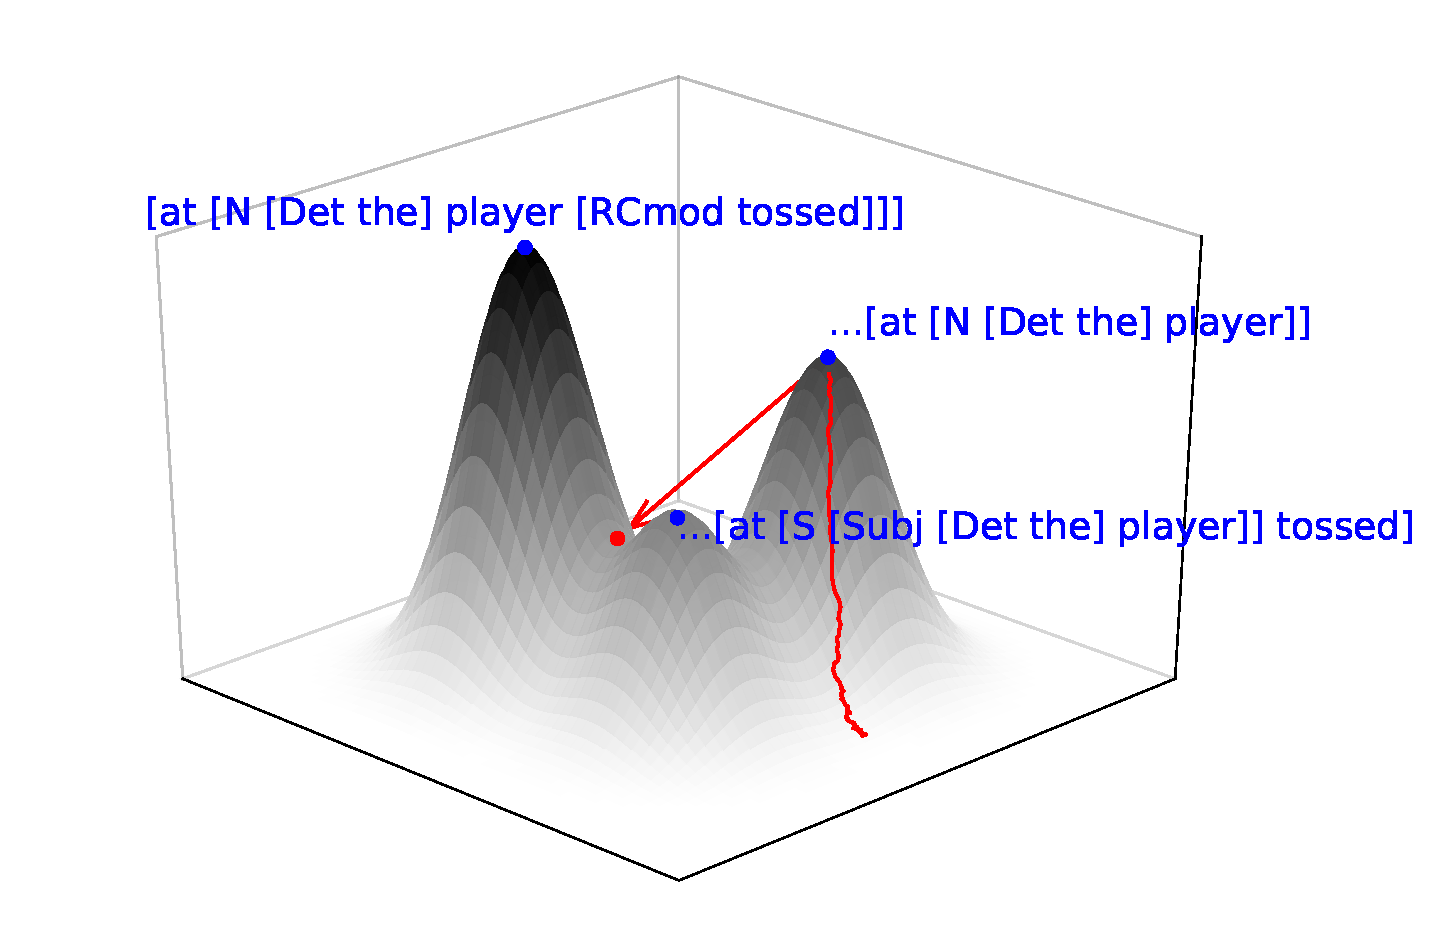
\includegraphics[width=\linewidth]{../Figures/ToyHarmonySurface.pdf}
\label{IllustrativePotentialSurface}
\caption{A partial harmony surface for English. The vertical axis is harmony, and the other two dimensions code feature/link configurations. After reading \emph{the coach smiled at the player}, the system follows the trajectory shown in read. The system dynamics drive it to build a well-formed partial parse with \emph{the player} attached as the nominal dependent of \emph{at} at the peak labeled [at [N [Det the] player]. Once it has stabilized on that structure, \emph{tossed} is read, jumping the system (red arrow) to a point intermediate between the grammatical [at [N [Det the] player [RCmod tossed]]] and the locally coherent but low-harmony [at [S [Subj [Det the] player] tossed]. From there, the system will settle again until it gets close enough to one of the peaks, then the process repeats.} 
\end{figure}

%In the analysis of local coherence effects we present below, we show that, for a wide range of plausible parameter settings, the system shows the observed interference phenomenon, and for a smaller, but non-negligible range of parameter settings the system shows competition-based facilitation. We note that this latter effect may offer insight into another phenomenon---the much puzzled-over ambiguity advantage effect \cite{traxler1998adjunct}. 

%As discussed below, we employ a systematic method of deriving the harmony function from \sout{a parsed corpus of sentences} local information about structural goodness. In this way, the framework offers a unified approach to a range of psycholinguistic phenomena, grounded in established linguistic insights about the structures of a wide range of sentences. Notably, like the surprisal theories \cite{hale2001probabilistic, levy2008expectation} but unlike a number of other sentence processing models \cite{Kimball19XX, Frazier1988, Gibson1991, Eberhardt2005, lewis2005activation}, the approach does not employ a set of parsing-specific additions to grammatical theory intended to address cases of parsing failure. Instead, parsing failure is an occasional, but natural outcome of the core structure building process itself---the process that discovers interpretations of word-sequence input.  

%Finally, although we do not focus on prediction in the current paper, SOSP offers a natural account of the many circumstances where the surprisal model correctly predicts differential reading times: harmony maximization drives the system to pre-activate features that are consistent with the input observed thus far---this is an example of the well-known pattern-completion property of neural networks and other self-organizing systems \cite{haken2004synergetic, BishopPatternCompletion}. Consequently, if the input introduces features that conflict with a pattern that has been partially or fully completed, the state can be bumped into a flat region between peaks (reflecting the equivocalness of the information it has received), and it will generally take a long time to stabilize again, predicting high processing times in cases of high surprisal.

We first present our SOSP framework and show how it makes timing predictions. We then turn to an implemented model SOSP model of local coherence effects, illustrating the principles just outlined. Finally, we conclude with a discussion of how SOSP relates to existing theories of sentence processing.

%[Note:  I think we should illustrate a complex case in a sketchy way in Figures 1stTreeletFigure and IllustrativePotentialSurface.  We should also acknowledge this complex structure by indicating some of its parts, when, further down in the paper, we introduce the 2-dimensional model.]

%[Note:  this intro does not provide any detail on the "systematic way of deriving the potential function from a parsed corpus".  The main body should therefore lay out, in brief form, the principles of this before illustrating with the specific example]

%[Note:  This introduction focuses on the relation to surprisal.  This means the General Discussion should give important words to ACT-R and to GSC.  ACT-R is an interesting case:  it doesn't fully enforce grammar-supervision (e.g., cue-based retrieval allows certain divergences...); however, it nevertheless enforces grammar-supervision where local coherence is concerned because (I think) it assumes that only structures that fit with the current parse structure are added on (check Lewis \& Vasishth).]
%	
%--------
%
%\begin{figure}[h!]
%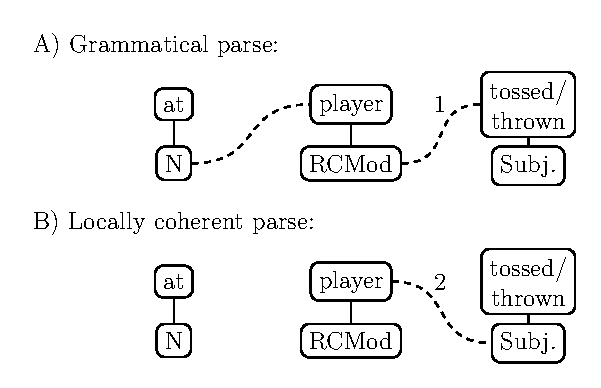
\includegraphics[width=\linewidth]{./Figures/LocalCoherenceStructs.pdf}
%\caption{Dependency structures assumed to model \citeA{tabor2004effects}. Panel A shows the gramatical parse: The preposition \emph{at} takes \emph{player} as its nominal dependent, and \emph{player} takes the participle as the head of a relative clause modifier. Panel B shows the ungrammatical, locally coherent parse in which \emph{at} fails to attach anything as its dependent, and the participle takes \emph{player} as its subject dependent. The numbers on the links are used to label the links in the simulations below.}
%\label{deps}
%\end{figure}

\section{A new formalization of SOSP}
In SOSP, linguistic structures are built out of lexically anchored syntactic treelets. The treelets connect with each other via graded attachment links (Fig.~\ref{1stTreeletFigure}). We assume for simplicity a dependency grammar formalism \cite<e.g.,>{hudson2007language, mcdonald2013universal}, so the only attachment sites are ones allowing a word to attach as the dependent of another word (\emph{head} attachment sites) and ones that allow other words to attach as dependents (\emph{dependent} attachment sites). The head and dependent attachment sites on each treelet are feature vectors encoding syntactic and semantic properties of a word and its expected dependents, respectively. Some features can change (e.g., the number marking on the determiner \emph{the} depends on the number of its licensor), and others are fixed in the lexicon. The only constraints on which links can form are that 1) no links can form within a single treelet (e.g., a determiner dependent site on a noun cannot link to the head of that same noun), 2) links can only form between head attachment sites dependent attachment sites, i.e., no head-head or dependent-dependent links can form.\footnote{We allow links to fail to form, creating partial, fragmentary structures, however, these parses are penalized and receive lower local harmony.}%, and \textbf{3) all words must be attached as the dependent of another treelet}\footnote{The matrix verb of a sentence attaches as the dependent of a special root node that is not subject to this requirement.}. 
All other links, grammatical and ungrammatical, are allowed to form. %For example, a link can form between the head attachment site of a verb to the determiner attachment site on a noun, which would amount to saying that the verb is the noun's determiner.

To facilitate intuitive interpretation of the values on each dimension, we use the convention of placing linguistic structures at the corners of the unit hypercube (0 = feature or link off, 1 = on). In order to allow multiple tokens of the same treelet in one sentence (e.g., \emph{the} in \emph{the dog saw the cat}), all of a treelet's dimensions are repeated for every position in a sentence. Thus, there is a set of dimensions corresonding to \emph{the} as the first word of a sentence, a different set of dimensions for \emph{the} as the second word, etc. Links are therefore between sentence-position-specific instances of treelets. 

Not all attachment links make equally well-formed structures, though. Structures in which all linked feature vectors are perfectly matched receive the highest possible harmony value of 1. Any feature mismatch results in a lower harmony value for that structure. In this way, SOSP implements a graded notion of well-formedness.We quantify the local harmony $h_i$ of a (partial) lingustics structure $i$, i.e., degree of well-formedness for $i$'s configuration of features and links, using Eq.~\ref{local_harmony}:%, which build on \citeA{smolensky1986information}'s formulation of the local harmony $h_i$ of a (partial) linguistic structure $i$:
%\begin{equation}\label{local_harmony}
%h_i = \prod_{l\in links} \frac{\vert\rho(\mathbf{f}_{l, head})^\intercal \rho(\mathbf{f}_{l, dependent})\vert}{len(\mathbf{f}_{l, head})}
%\end{equation}
\begin{equation}\label{local_harmony}
h_i = \prod_{l\in links}  \tfrac{dist(\mathbf{f}_{l, head})^\intercal \rho(\mathbf{f}_{l, dependent})}{len(\mathbf{f}_{l, head})}
\end{equation}
The local harmony $h_i$ of a structure is the product of the Hamming distance $dist(\cdot)$  between the \sout{absolute value ($\vert\cdot\vert$) of the dot product of the} feature vectors at the head $\mathbf{f}_{l, head}$ and dependent $\mathbf{f}_{l, dependent}$ ends of each link $l$ scaled by the length of the feature vectors ($len(\cdot)$). %The function $\rho(z) = 2z - 1$ maps the feature vectors element-wise from [0, 1] to [-1, 1], which makes the numerator in %where +1 means a feature is ``on,'' -1 means ``off,'' and 0 means not specified in the lexicon.
This definition of local harmony is valid for any combination of features and links, even those that strongly violate rules of a symbolic grammar, e.g., the clash structure [\emph{at} [S [Subj [Det \emph{the}] \emph{player}] \emph{tossed}\dots]]). In the simulations below, we will see that the presence of these lower-harmony structures in the mental representation of possible structures plays a key role in explaining observed timing effects.

Eq.~\ref{local_harmony} allows us to calculate the harmony of any linguistic configuration, but on their own, the $h_i$s do not tell us how to choose a structure given the input. Thus, we need a way of relating the different structures and a mechanism for navigating among them given some input. %Since the $h_i$ encode a person's knowledge of the well-formedness of different possible structures, we need a way for the parser to navigate among the different structures and locally maximize harmony given its input. To do this, we relate different parses by defining a harmony landscape on which the system navigates as it tries to find the best possible structure by local optimization. This harmony landscape was designed to assign well-formedness values for structures intermediate between discrete, symbolic linguistic structures while ensuring that  structures are the only attractors of the system (i.e., points to which the system will return after a small perturbation, \citeA{strogatz1994nonlinear}). %In comprehension, a word being read is modeled as switching on the relevant features in the correct position in a sentence and allowing the system to settle to the nearest attractor.

\subsection{Defining the harmony landscape and dynamics}
%An SOSP parser should maximize the harmony of the structure it builds given its input; in other words, it should perform hillclimbing on a harmony landscape where the hilltops correspond to structures of varying degrees of well-formendness. Eq.~\ref{local_harmony} only tells us how high a harmony peak should be, but not where it is or how to get there. 
A simple method for defining where the peaks in our harmony function should be is to use a sum of radial basis functions (RBFs) $\phi_i$ \cite{han1989convergence, ciocoiu1996analog, ciocoiu2009invariant, muezzinoglu2006rbf}:
$$
\phi_i(\mathbf{x}) = \exp\left(-\tfrac{(\mathbf{x} - \mathbf{c}_i)^\intercal(\mathbf{x} - \mathbf{c}_i)}{\gamma}\right)
$$
Here, $\mathbf{x}$ (a column vector) is the $d$-dimensional state of the system encoding values of all features and links in $\mathbb{R}^d$, each $\mathbf{c}_i$ is the location of the $i$th (partial) parse (encoding desired feature values and link strengths), $^\intercal$ denotes the vector transpose\footnote{Note that $(\mathbf{x} - \mathbf{c}_i)^\intercal(\mathbf{x} - \mathbf{c}_i)$ is equivalent to the square of the Euclidean distance between $\mathbf{x}$ and $\mathbf{c}_i$.}, and $\gamma$ (a free parameter) sets the width of the RBFs. We then define the harmony function $H(\mathbf{x})$ as the sum of $n$ RBFs, where $n$ is the number of partial and full parses (harmony peaks) we wish to encode:
\begin{equation}\label{harmony}
H(\mathbf{x}) = \sum_{i}^{n} h_i \phi_i(\mathbf{x})
\end{equation}
where the $h_i$ give the local harmony of a (partial) parse, computed using Eq.~\ref{local_harmony}. This equation creates the hilly harmony landscape mentioned above, assigning harmony values both to the $\mathbf{c}_i$ and to all states intermediate between them.\footnote{One question that arises with this system is what parameter settings ensure separate harmony peaks for each $\mathbf{c}_i$. Exploratory simulations and numerical bifurcation analyses \cite{meijer2009numerical} using a one-dimensional system with peaks at $x = 0$ and $x = 1$ suggest that the harmony peaks remain separate as long as $\gamma$ is small enough. When the $h_i$ are equal, there is a pitchfork bifurcation at $\gamma = 0.5$, when the two separate harmony peaks merge into a single peak halfway between the $\mathbf{c}_i$ \cite[report a similar finding]{muezzinoglu2006rbf}. For unequal $h_i$, the system exhibits a cusp bifurcation, with the lower-harmony peak being absorbed into the larger harmony peak for values of $\gamma$ that, in general, are lower than 0.5. As discussed below, even if the lower harmony parse does not have a separate peak, it can still affect parsing by warping the harmony surface and thereby deflecting trajectories from a more direct path to an attractor. A more systematic exploration of the parameter space is left to future work, but these explorations allow us constrain $\gamma$ and the $h_i$ somewhat in our simulations.}\label{bif}

In SOSP, treelets are interacting subsystems that ``attempt'' to assemble themselves through local interactions to locally maximize the harmony of the resulting structure. Since the gradient of a scalar-valued function like $H(\mathbf{x})$ points in the direction of steepest ascent, we make the system change in time so that it follows this gradient uphill in a noisy way:
\begin{equation}\label{dyn}
\frac{d\mathbf{x}}{dt} = \nabla_\mathbf{x} H(\mathbf{x}) = -\tfrac{2}{\gamma} \sum_{i}^{n} h_i (\mathbf{x} - \mathbf{c}_i) \phi_i(\mathbf{x}) + \sqrt{2D}\ dW
\end{equation}
$D$ scales the magnitude of the Gaussian noise process $dW$. Gradient dynamical systems of this sort exhibit simple behavior: given an initial condition, the system simply settles into the nearest attractor (neglecting the effects of the noise) \cite{hirsch1974differential}. Because we choose the locations of the (partial) parses $\mathbf{c}_i$, this setup guarantees that the system will settle into one of the pre-programmed attractors that corresponds to a symbolic structure, as long as the parameters are set so that all of the $\mathbf{c}_i$ exist as separate harmony peaks. %(We leave the question of learning the $\mathbf{c}_i$ to future research).

The approach in Eqs.~\ref{local_harmony}-\ref{dyn} can be applied to any linguistic structure describable in terms of features and attachment links, making SOSP a general theory of sentence processing. The parsing dynamics are derived directly from the harmony function, so SOSP provides a direct mapping between the well-formedness of linguistic structures and how the system will behave when parsing that structure. We now show how this feature of SOSP leads directly to predictions about processing times.

\subsection{Predicting processing times}
There are several ways to illustrate how settling times depend on the harmony of the parse that forms. To illustrate, we will first consider the simplest possible case, a one-dimensional system with a single harmony peak at $x = 0$. The harmony function is $H(x) = h~\phi(x) = h~\exp\left(-\tfrac{x^2}{\gamma} \right)$ and the dynamics are given by $\dot{x} = -\tfrac{2h}{\gamma}~x~\phi(x)$.
%\begin{equation}\label{dyn1d}
%\dot{x} = -\tfrac{2h}{\gamma}~x~\phi(x)$.
%\end{equation}
From this equation, we can already see that the higher the harmony of the attractor, the faster system moves toward it. Another way of seeing this is to consider the time $dt$ it takes to travel an infinitesimal distance $dx$,
\begin{equation}\label{dt}
dt  = dx/\dot{x} = \left(-\tfrac{2h}{\gamma}~x~\phi(x)\right)^{-1}~dx,
\end{equation}
since time equals distance divided by velocity. To find the time $t_s$ to settle the from an initial point $x_0$ at $t = 0$ to a point $x_1$ near the attractor at $x = 0$\footnote{It takes infinitely long to actually reach $x = 0$, so we make $x_1$ offset a small amount from the fixed point so the integral converges.}, we can simply integrate both sides of Eq.~\ref{dt}:
\begin{align}\label{ts}
\int_{0}^{t_s} dt & = \int_{x_0}^{x_1} \left(-\tfrac{2h}{\gamma}~x~\phi(x)\right)^{-1}~dx \nonumber \\
t_s & = \tfrac{\gamma}{2h} \int_{x_0}^{x_1} -\frac{1}{x}\exp\left(\tfrac{x^2}{\gamma} \right)~dx \nonumber \\
t_s & \propto (2h)^{-1}
\end{align}
Thus, the time it takes to settle to a point close to the attractor in this 1D system is inversely proportional to two times the harmony of the structure. (The integral on the rhs. can be calculated numerically, and since we use the same $\gamma$ for all attractors, its effect on settling times is constant%\textbf{. Note to Whit: the analytical solution to this integral involves exponential integrals, a special function defined as the integral of the ratio of exp(x) to its derivative, so it's not very informative.})
. The relation between well-formedness and settling times is therefore quite simple: well-formed structures are faster to build than ill-formed structures.

In general, though, an SOSP parser will have many dimensions coding multiple features and link strengths, and there will be many attractors corresponding to the different structures that can form. Does something like Eq.~\ref{ts} hold in the general case? %We assume that 
Once the system has entered the basin of attraction for a particular attractor, the \sout{most relevant} strongest force acting on the system is the pull of that attractor; the effects of all of the other $\mathbf{c}_i$ drop off exponentially. As an approximation, we can simplify Eq.~\ref{dyn} so that the only element in the sum is the on for the selected attractor, similar to Eq.~\ref{dyn1d}. From there, it is simple to see that the same relation between settling time and harmony in Eq.~\ref{dt} holds\footnote{For $d > 1$, the integral in Eq.~\ref{ts} needs to be replaced with a line integral connecting the initial and final conditions.}$^,$\footnote{Yet another way of seeing the dependence of settling times on the local harmony is to find the characteristic time scale of the attractor \cite{strogatz1994nonlinear}, which involves finding the eigenvalues of its Jacobian matrix (linearization) and taking the reciprocal of the largest of them (all eigenvalues of an attractor are negative). For Eq.~\ref{dyn1d}, the linearization is $\dot{x} = -(2h/\gamma)x$, so the characteristic time scale is $\gamma / 2h$, as in Eq.~\ref{ts}.}. However, the effects of other attractors are, in general, not completely negligible. As illustrated in Fig.~\ref{harmonylandscape}, the presence of a relatively high-harmony attractor can temporarily bow trajectories away from an attractor by warping the harmony landscape, even though the system is not in the basin of attraction of the lower-harmony competitor. So, within the basin of attraction of a particular parse, the settling time is approximately inversely proportional to double the harmony of that parse, modulo the noise and this bowing.

Word-by-word parsing works by turning on the features of a word at a particular position in the sentence. This places the state of the system away from an attractor, since attractors correspond to stable configurations of features \emph{and} links, and the input leaves the links untouched (i.e., at zero strength). The system then settles towards one of the nearby attractors according to the harmony gradient and the noise. Over repeated trials, the noise will drive the system to settle into different parses. %The overall mean settling time at a given word is then the mean of the settling times to each attractor chosen weighted by how often the system chooses that attractor. 
Thus, the theory of timing in SOSP is this: the local harmony of different structures determines approximately how fast that structure forms (modulo noise and trajectory bowing from competing attractors), and the average processing time at a given word over many trials is the weighted average of the settling times to each parse chosen. We now illustrate how this works using a simple model of local coherence effects.

\section{A simple SOSP model of local coherence effects}
A full model of the word-by-word processing of the sentences in \ref{LCegs} would involve incrementally turning on features of the first word \emph{the}, allowing the system to settle to the nearest attractor, then turning on the features of \emph{coach}, and repeating until the end of the sentence. We can model the main local coherence finding from \citeA{tabor2004effects}, however, by assuming that the parser has already read up to \emph{The coach smiled at the player tossed/thrown\dots} and that the main settling that still has to be done is choosing how to attach \emph{player} and \emph{tossed/thrown}, as shown in Fig.~\ref{1stTreeletFigure}. We do this using a two dimensional system:
\begin{equation}
\begin{aligned}\label{2dlc}
\phi_1(x_1, x_2) &= \exp\left(\tfrac{(x_1 - 1)^2 + x_2^2}{\gamma}\right)\\
\phi_2(x_1, x_2) &= \exp\left(\tfrac{x_1^2 + (x_2 - 1)^2}{\gamma}\right)\\
\dot{x_1} &= -\tfrac{2}{\gamma}(h_1 (x_1 - 1) \phi_1(x_1, x_2) \\ &+ h_2 x_1 \phi_2(x_1, x_2)) + \sqrt{2D}~dW_1\\
\dot{x_2} &= -\tfrac{2}{\gamma}(h_1 x_2 \phi_1(x_1, x_2) \\ &+ h_2 (x_2 - 1) \phi_2(x_1, x_2)) + \sqrt{2D}~dW_2
\end{aligned}
\end{equation}
The two dimensions ($x_1$ and $x_2$) are the strength of the \emph{tossed/thrown-player} link (fully grammatical with \emph{player} as the head of the participle; link 1 in Fig.~\ref{1stTreeletFigure}) and the strength of the \emph{player-tossed/thrown} link (ungrammatical, with \emph{player} as the subject dependent of \emph{tossed/thrown} coerced to be a main verb; link 2 in Fig.~\ref{1stTreeletFigure}). We need only two attractors in the system: one at [1, 0], which is the correct, maximal-harmony parse, and one at [0, 1], which will have different sub-maximal harmonies depending on whether \emph{tossed} or \emph{thrown} has been read (see Fig.~\ref{harmonylandscape}). Because \emph{player} is a good feature match to be the subject of \emph{tossed} (when interpreted as an active verb), the attractor at [0, 1] is penalized only for having a missing link between \emph{at} and \emph{player}. For \emph{thrown}, though, [0, 1] is additionally penalized because the features on the participle \emph{thrown} do not match \emph{player}'s feature that specifies that it should be dependent on a main verb. \textbf{Why else should it be penalized?}. We assume that the system starts at [0, 0], reflecting the assumption that only the links connecting the words need to develop. %The settling time of the model is taken to reflect the amount of time it takes for the mind to integrate these words in to a linked syntactic structure.

\begin{figure}[h!]
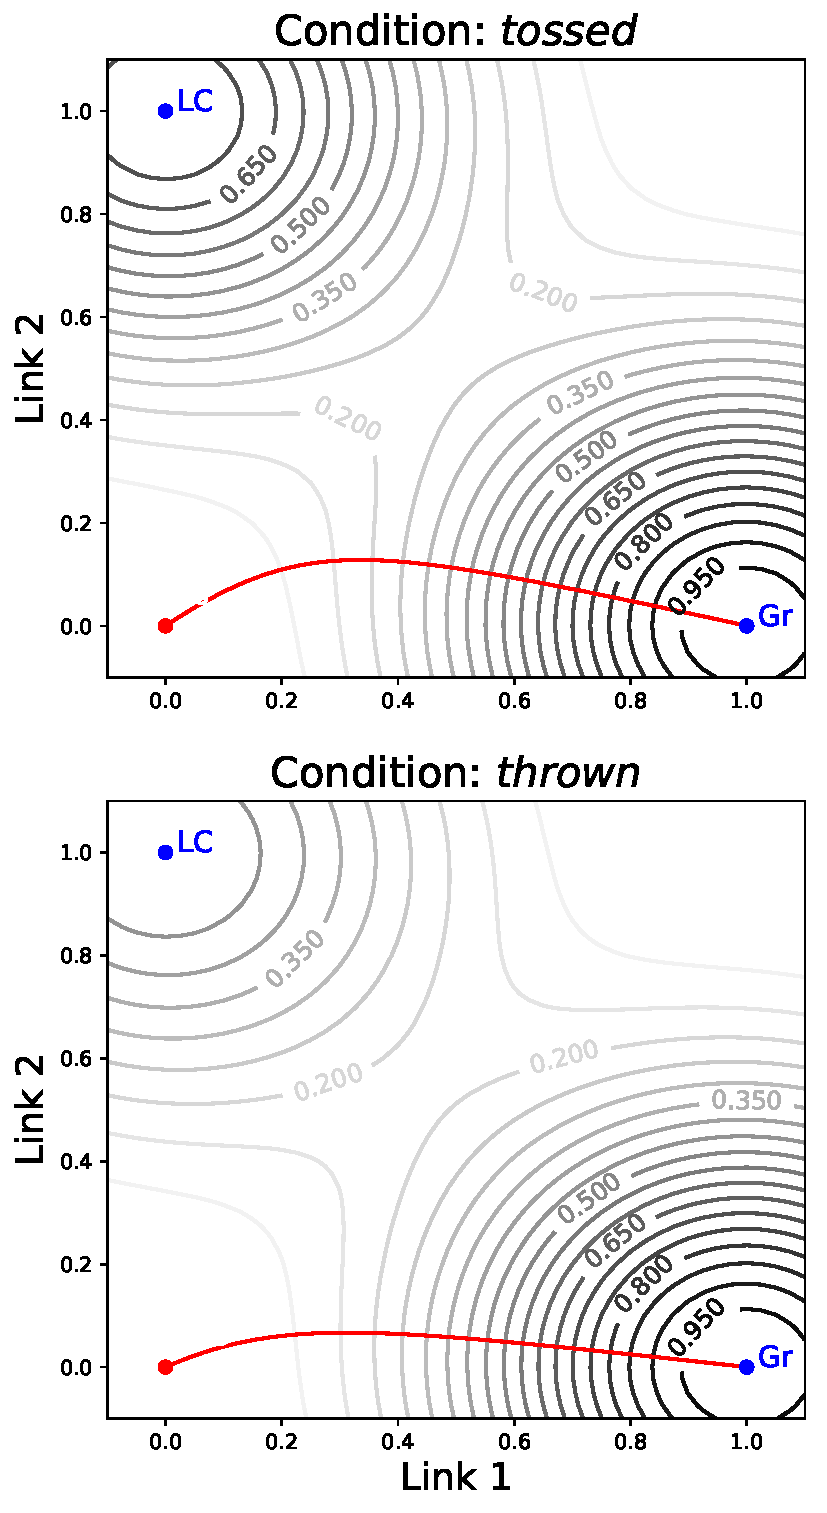
\includegraphics[width=0.8\linewidth]{../Model/HarmonyContours.pdf}
\centering
\caption{Contour plots of the harmony landscapes. Contour labels give the harmony at that level. Red lines show noiseless trajectories starting from [0, 0] and approaching the grammatical parse (Gr) at [1, 0]. Note how the trajectory for \emph{tossed} is more bowed toward the locally coherent attractor (LC; causing extra slowdown) compared to \emph{thrown}.}
\label{harmonylandscape}
\end{figure}

We simulated both conditions 2000 times using Euler forward discretization with a time step of 0.01. The noise magnitude $D$ was set to 0.001, and $\gamma$ was 0.25. The system ran until it got within a small radius of an attractor. For illustration purposes, the local harmony $h_1$ of the locally coherent attractor ([0, 1]) was set to 0.75 in the \emph{tossed} condition, and in the \emph{thrown} condition to 0.5 (see below for a more systematic investigation of $h_1$'s effect). %Paralleling the human data in \citeA{tabor2004effects}, the theory above predicts that the \emph{tossed} condition should be slower than the \emph{thrown} condition on average. 
SOSP predicts that, for both \emph{tossed} and \emph{thrown}, the noise should bump the system towards the grammatical parse in most cases because its high harmony dominates the harmony landscape. When the noise does push the state towards the locally coherent attractor, it will approach it more slowly in the \emph{thrown} condition than in the \emph{tossed} condition because of \emph{thrown}'s lower harmony. But because this happens so rarely, the average time will be dominated by fast approaches to the grammatical attractor. The low-harmony parse for \emph{tossed} will be selected more often, though, due to its higher harmony, so it will pull the average settling time down more than the \emph{thrown} condition. Thus, the presence of a relatively high-harmony competitor for the grammatical parse will cause a competition-based slowdown averaged over many trials.

As predicted, the system settled into the ungrammatical attractor in both cases, and it did so more frequently in the \emph{tossed} condition (about 12\% of runs) than in the \emph{thrown} condition ($<$1\% of runs). This caused the average settling time to be higher for \emph{tossed} (in time steps: $M = 158.588, SD = 28.133$) than for \emph{thrown} ($M = 149.459 SD = 25.576$), paralleling the results of \citeA{tabor2004effects}.

These simulations are based on the assumption that the local harmony of the locally coherent parse is higher for \emph{tossed} than \emph{thrown}, making the former a stronger competitor than the latter. However, it is not immediately clear which features are relevant for calculating the $h_i$ such that this relation holds.\footnote{Future work will seek to learn relevant dependency-specific features from a large corpus \cite{zhao2014learning, bansal2015dependency}, which will open the door to broad-coverage analyses of reading times similar to \citeA{smith2013effect} and \citeA{engelmann2018effect}.} For now, we plot mean settling times as a function of the harmony $h_1$ of the ungrammatical parse (Fig.~\ref{fnofh1}). We used $\gamma = 0.25$ here, but this pattern holds for a wide range of $\gamma$ values. This figure shows that there is broad range of $h_1$ values such that as long as the \emph{tossed} condition has a higher $h_1$ than the \emph{thrown} condition, we will observe local coherence effects. Thus, local coherence effects are generally predicted whenever we compare higher- and lower-harmony competitors for a grammatical parse, a result supported by the large-scale eye-tracking corpus study of \citeA{bicknell2009correcting}.

Something interesting happens when $h_1$ is greater than about 0.85, though. As $h_1$ increases beyond that point, the average settling times start to drop. The bottom panel of Fig.~\ref{fnofh1} suggests why: as the competing ungrammatical parse increases in harmony, the time it takes the system to settle to it approaches that of the grammatical parse, so it no longer pushes the overall average settling time up as much. In this range of $h_1$ values, there is still a slowdown due to competition, but it is not as large as the slowdowns observed for somewhat lower-harmony competitors. In effect, the model predicts that we should observe the strongest competition-induced slowdowns when the competing structure is of moderate harmony, and that we should observe smaller-magnitude slowdowns for both very low harmony competitors, and (to a lesser extent) higher harmony competitors. This behavior is, to our knowledge, unique among models of sentence processing. We speculate that this property of SOSP might provide a new explanation for the ambiguity advantage \cite[e.g.]{traxler1998adjunct}, where certain ambiguous relative clause and adjunct attachments are  read more quickly than comparable unambiguous structures. This effect has been argued to rule out competition-based theories of parsing, but if the $h_i$ of both parses are close to 1 in the ambiguous condition but one is appreciably less than one in the unambiguous conditions, the competition-based SOSP might be able to explain this otherwise puzzling effect. %Future work will explore whether this property of SOSP can indeed explain the observed effects.

\begin{figure}[h!]
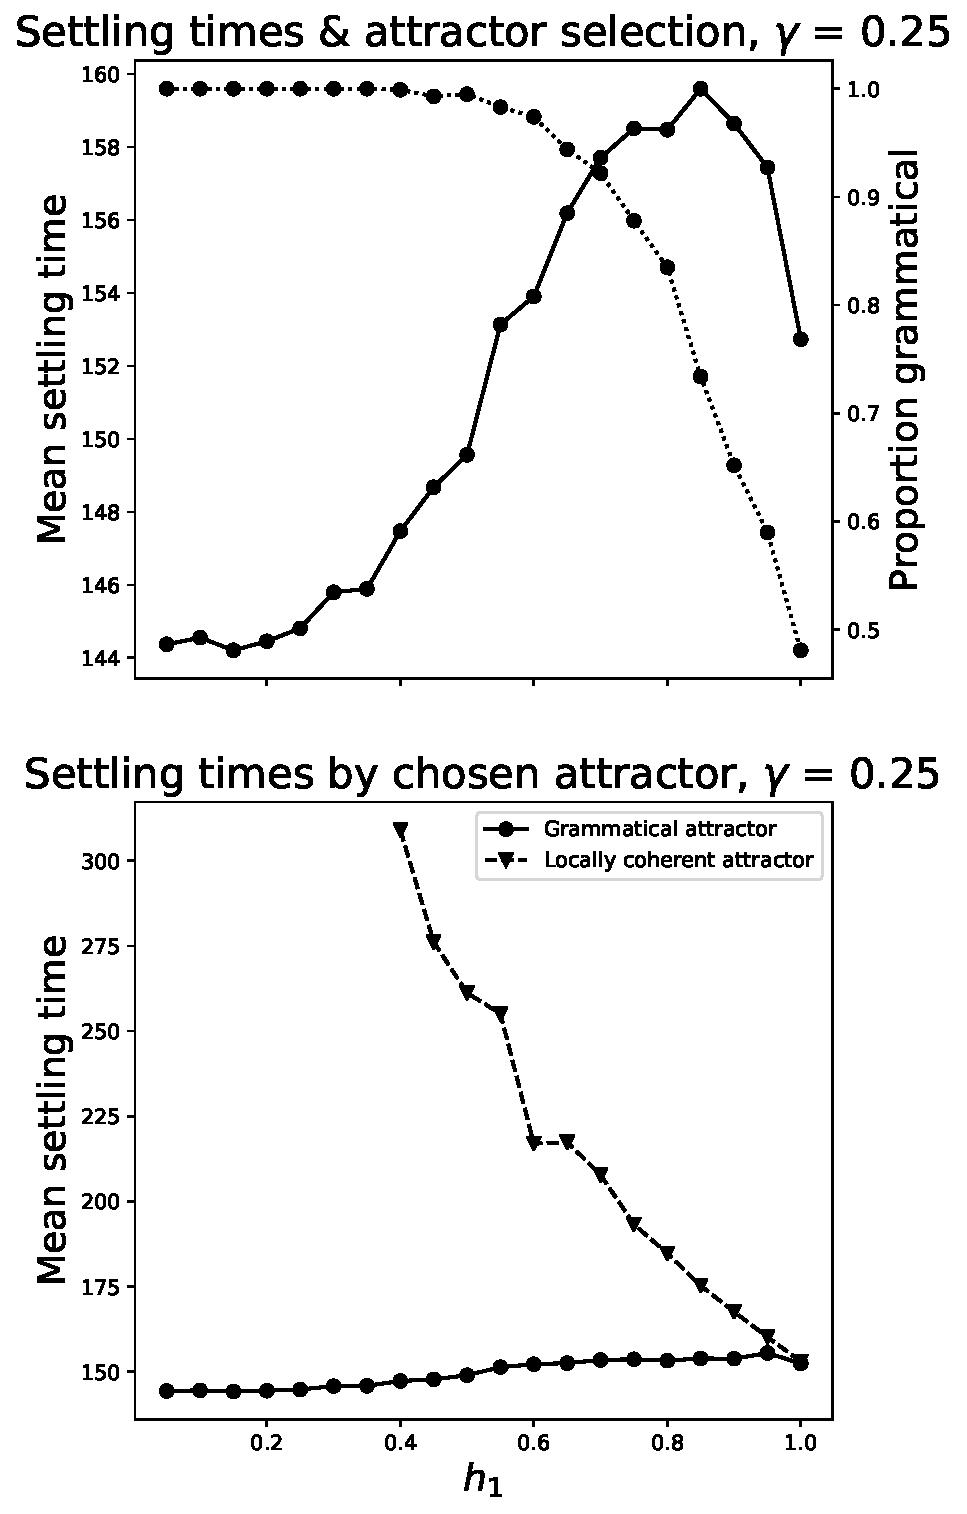
\includegraphics[width=0.8\linewidth]{../Model/TimesAsFnOfH1.pdf}
\centering
\caption{Top panel: mean settling times for the local coherence model as a function of the ungrammatical parse $h_1$ (solid line, left y-axis) and the proportion of runs in which the system selected the grammatical parse (dotted line, right y-axis). Bottom panel: mean settling time by selected parse (solid line and circles = grammatical, dashed line and triangles = locally coherent parse). For $h_1 < 0.4$, the system never settled on the ungrammatical attractor,  likely because that attractor does not exist below that point (see footnote \ref{bif}).}
\label{fnofh1}
\end{figure}

\section{Discussion}
In this paper, we have introduced a theory of timing effects in a self-organizing sentence processing (SOSP) framework and demonstrated how it can explain the local coherence effects first presented in \cite{tabor2004effects}. In SOSP, the amount of time it takes to build a structure depends on how well-formed the structure is, and the average structure-building time over many trials is the weighted average of settling times to each parse chosen.\footnote{The weighted averaging feature of SOSP is quite similar to recent similarity-based interference approaches building on \citeA{lewis2005activation} that model reading time effects as statistical hierarchical mixture models \cite{nicenboim2018models, vasishth2017feature}.} We showed how this theory is derived directly from the equations of SOSP, which were designed to locally find the highest-harmony structure given the input in a harmony landscape that contains both low- and high-harmony structures as attractors.

In the local coherence model, the lower-harmony attractors in the harmony landscape played a key role: A relatively strong but ungrammatical (and therefore slow-to-build) competitor slowed settling more than a weaker ungrammatical competitor because the stronger competitor was built more often. This account differs from the noisy channel approach to local coherence \cite{levy2009eye}, where it is assumed that the parser can edit its input to preserve grammaticality \cite[provide a similar approach in a dynamical, harmony based model]{cho2017incremental}. In this way, SOSP is different from grammar supervision theories of sentence processing, where only grammatical structures are considered, e.g., surprisal theory as calculated from probabilistic symbolic grammars \cite{levy2008expectation, hale2001probabilistic}. Also, like surprisal but unlike a number of other sentence processing models \cite{kimball1973seven, frazier1978sausage, gibson1991computational, eberhard2005making, lewis2005activation}, the approach does not add anything to grammatical theory to avoid or repair parsing failure. Instead, parsing failure is an occasional, but natural outcome of the core structure building process itself---the process that discovers interpretations of word-sequence input. SOSP therefore offers a unique and parsimonious approach to sentence processing: Ungrammatical structures not play a key role in successful and unsuccessful parses, they obviate the need for processing mechanisms other than local harmony maximization. %and even the harmony-based Gradient Symobolic Computation \cite<GSC; at least as it has been presented so far;>{cho2016bifurcation, cho2017incremental, cho2018dynamic}. 

%The simulations shown in Fig.~\ref{fnofh1} show that SOSP predicts local coherence effects for a broad range of parameter settings: Higher-harmony competitors will be slower than lower-harmony competitors. For very high-harmony competitors, the pattern is different, though. SOSP predicts that sentences with very high-harmony competitors will actually be faster than sentences with medium-harmony competitors. This property might have application to the ambiguity advantage, which we leave to future research. A similar SOSP model was shown to predict subject-verb number agreement patterns in English pseudopartitives (\emph{a pile of sandwiches is/are on the table\dots}, and the SOSP framework has been argued to explain encoding interference effects in English and Italian \cite{villata2018encoding}. The present work extends the range of empirical phenomena that SOSP can explain and greatly generalizes the mathematical framework. If SOSP can indeed capture all of these effects, it would strongly support SOSP as a general theory of sentence processing.

%\textbf{Add discussion of GSC}

%Discuss the relationship to Pyeong Whan's recent models. \citeA{cho2018dynamic} show that processing times in their system will be proportional to surprisal (which for them is $\Delta H$), but for us, since the input starts the system away from a (partial) parse, that this is not the same as surprisal as defined in \citeA{hale2001probabilistic, levy2008expectation}.

%Future directions: using better methods for predicting settling times, especially a way of mapping time in the model to time in actual experiments. Also, \citeA{gardiner1985handbook}, section 9.3 seems promising. In particular, long-term behavior of sys. (st. prob. distr. which is soln. of Fokker-Planck eq.) shows that the mind is vastly more likely to settle into the highest-harmony states \cite{smolensky1986information}. However, on-line processing is all about transients, where the tools are hairier mathematically...

\section{Acknowledgments}
This project was supported in part by NSF IGERT grant DGE-1144399. \textbf{others?}

\bibliographystyle{apacite}
\setlength{\bibleftmargin}{.125in}
\setlength{\bibindent}{-\bibleftmargin}
\bibliography{master}
\end{document}

%Our focus on timing effects here is motivated by the fact that previous dynamical parsers like SOSP have had little success in predicting timing data, despite the fact that time plays such a central role in these models---they are all implemented as sets of differential equations or iterated maps which describe how the state of a parse changes in time. The dynamical models of \citeA{kempen1989incremental, vosse2009unification, tabor2004evidence} derive some timing predictions for a handful of phenomena via direct simulations, however, a relatively large number of other models \cite{vandervelde2006neural, vosse2000syntactic, cho2016bifurcation, cho2017incremental, smith2018self, gerth2009unifying} either do not make timing predictions or the timing predictions are not discussed. More importantly, though, there is no theory of why processing one structure should take longer than another structure in these frameworks. In the SOSP framework we present, timing effects are shown to be directly related to the well-formedness (harmony) \cite{smolensky1986information} of the linguistic structure that is built: Sentence structures that are less well-formed take longer to process than more well-formed structures, and the overall average settling time (comparable to averages calculated from experiments) is average of the settling times to each parse chosen weighted by how frequently that parse is selected. While this result seems intuitive, we show below how it follows directly from the calculation of harmony and the dynamical equations that govern how the system parses. Moreover, it makes novel testable predictions that, to our knowledge, are unique among extant theories of sentence processing.

%We note that one very promising related result is presented in \citeA{cho2018dynamic}, where Cho et al. show that, in a related but different dynamical parser (Gradient Symbolic Computation, GSC), the change in harmony from one parsing step to the next is equivalent to surprisal, which is known to predict reading times over a large range of word predictability \cite{hale2001probabilistic, levy2008expectation, smith2013effect}. This effort is closely related to the present paper, but it differs in that GSC only grammatical structures to stabilize by the end of a sentence. In SOSP, allowing the system to stabilize on ungrammatical structures will be key to explaining local coherence effects.

%Most of the time, people produce and interpret sentences according to the rules of some grammar. However, they sometimes temporarily entertain or even settle on structures that are not completely faithful to those rules. Here, we introduce self-organizing sentence processing (SOSP) \cite{smith2018self} as a general theory of reading time effects that we then apply to an interesting case of ``grammar flouting'' interference in sentence comprehension.

%We consider local coherence effects \cite{tabor2004effects, konieczny2005psychological, paape2015local, bicknell2009correcting, levy2009eye}, where the parser seems to entertain a locally coherent structure that is incompatible with the rest of the sentence. For example, \citeA{tabor2004effects} used sentences like \emph{The coach smiled at the player \textbf{tossed/thrown} the frisbee\dots}. The sequence \emph{the player tossed the frisbee\dots}, on its own, is a grammatical sentence. However, the rest of the sentence in which it appears rules out this structure, since the preposition \emph{at} cannot grammatically take a sentence as its complement (*[PP \emph{at} [S \emph{the player tossed the frisbee\dots}]]). Tabor and colleagues found that participants read the region containing \emph{tossed} significantly longer than the corresponding region for \emph{thrown}, suggesting that the locally coherent but globally illicit parse was competing with the correct parse ([PP \emph{at} [NP \emph{the} [N' \emph{player} [VP \emph{tossed the frisbee}]]]]). This result suggests that people at least temporarily entertain ungrammatical parses and motivates a theory of parsing in which suboptimal structures can influence processing (unlike strictly rational approaches to sentence processing, as argued in, e.g., \citeA{levy2009eye}).

%If we can assume that once the system is in the basin of attraction of a particular $\mathbf{c}_i$, the effects of the other attractors is negligible, then we can show that the same relation between settling times and local harmony holds. The $\phi_i$ in Eq.~\ref{dyn} scale how strongly the system is pulled toward the $i$-th attractor. So, if $\phi_i$ becomes negligible, we can simplify Eq.~\ref{dyn} to have just a single element in the sum, similar to Eq.~\ref{dyn1d}. For our purposes, we say that the effect of $\phi_i$ is negligible if $\phi_i < \theta,\ 0 < \theta \ll 1$, since 1 is the minimal distance between attractors. If we denote $\sqrt{(\mathbf{x} - \mathbf{c}_i)^\intercal(\mathbf{x} - \mathbf{c}_i)}$ (the Euclidean distance) by $y$, then, after inserting $y$ into Eq.~\ref{dyn} and solving for $y$, $\phi_i$ will be negligible as long as $y > \sqrt{-\gamma~ln~\theta}$. For example, if we choose $\gamma = 0.25$ and $\theta = 0.1$, then the system should be a distance of at least $y \approx 0.759$ away from the $i$-th attractor for us to ignore the effects of that attractor. From there, it is simple to see that the same relation between settling time and harmony in Eq.~\ref{dt} holds\footnote{For $d > 1$, the integral in Eq.~\ref{ts} needs to be replaced with a line integral connecting the initial and final conditions.}$^,$\footnote{Yet another way of seeing the dependence of settling times on the local harmony is to find the characteristic time scale of the attractor \cite{strogatz1994nonlinear}. To find the characteristic time scale, we find the eigenvalues of its Jacobian matrix (linearization) and take the reciprocal of the largest of them (the attractor is stable, so all of its eigenvalues are negative). For Eq.~\ref{dyn1d}, the linearization is $\dot{x} = -(2h/\gamma)x$, so the characteristic time scale is $\gamma / 2h$, as in Eq.~\ref{ts}.}.


%The second example of grammar-flouting interference comes from studies of agreement attraction in comprehension. When asked to repeat a subject noun phrase and then complete the rest of the sentence, participants produce a verb that agrees in number with a noun other than the grammatical subject of the sentence, e.g., \emph{the key to the cabinets \textbf{are}\dots} \cite[among many others]{bock1991broken} in a small but reliable proportion of trials. In addition, \citeA{haskell2003conflicting} provided evidence that participants were slower to complete the sentence with a plural intervening noun (e.g., \emph{cabinets}) than with a singular (e.g., \emph{cabinet}). Together, the production and timing effects suggest that not only do participants temporarily entertain ungrammatical structures, they can sometimes stabilize on them long enough to actually produce them.

%To predict how long it will take to form a particular parse, we first assume that the input or the noise has placed the state of the system in the attractor basin of that parse. We then ask how long it takes for the system to settle from that initial state $\mathbf{x}_0$ to a point close to the attractor $\mathbf{x}_1 = \mathbf{x}^* - \epsilon \cdot \mathbf{x}_0$, where $\mathbf{x}_i^*$ is the $i$th attractor and $\epsilon$ is a small constant\footnote{$\mathbf{x}_1$ therefore lies on the line connecting $\mathbf{x}^*$ and $\mathbf{x}_0$.}. This change in state will be associated with a change in harmony $\Delta H = H(\mathbf{x}_1) - H(\mathbf{x}_0)$. We follow \citeA{cho2018dynamic} in noting that it will take the system some time $t_c$ to travel this distance (and make the corresponding change in harmony), giving:
%\begin{equation}
%\begin{split}
%\Delta H &= \int_0^{t_c} \frac{dH(\mathbf{x})}{dt}dt = \int_0^{t_c} \nabla_\mathbf{x} H(\mathbf{x})^\intercal \frac{d\mathbf{x}}{dt} dt \\ &= \int_0^{t_c} \Vert \nabla_\mathbf{x} H(\mathbf{x})\Vert^2 dt = t_c \Vert \nabla_\mathbf{x} H(\mathbf{x})\Vert^2
%\end{split}
%\end{equation}
%The notation $\Vert\cdot\Vert$ is the Euclidean norm. Rearranging and evaluating $\Vert \nabla_\mathbf{x} H(\mathbf{x})\Vert^2$ at $\mathbf{x}_1$, we find that the time to get close to the attractor is:
%\begin{equation}\label{time_pred}
%t_c = \frac{\Delta H}{\Vert \nabla_\mathbf{x} H(\mathbf{x}_1)\Vert^2}
%\end{equation}
%Because we are assuming that $\mathbf{x}_0$ is already in the basin of attraction of $\mathbf{x}_i^*$, the effects of the other $\phi_j,\ j \neq i$ in $H(\mathbf{x})$ will be negligible.\footnote{As long as $\gamma$ is set small enough, $\phi_j(\mathbf{x}_1)$ will be close to zero since $\mathbf{x}_1$ will be far from the center $\mathbf{c}_j$.}. Thus, the approximation:
%\begin{equation}
%t_c \approx \frac{\Delta H}{\Vert2 h_i \gamma^{-1} (\mathbf{x}_1 - \mathbf{c}_i) \phi_i(\mathbf{x}_1)\Vert^2} \propto h_i^{-1}
%\end{equation}
%shows that the time to settle to an attractor from an initial point inside its basin of attraction will be inversely proportional to the attractor's harmony $h_i$. In this way, SOSP (and possibly other similar systems like \citeA{cho2018dynamic}) derives processing times directly from the theory of well-formedness via the processing dynamics.
%
%Each attractor will have its own $t_c$, so the average processing time for a given condition is predicted to be proportional to the average of the $t_c$ for each attractor that the system settles to in that condition weighted by the probability of settling to that attractor.


%Ignoring the effect of noise, we can calculate the time $T_i$ it takes a system to move from some initial position $\mathbf{x}_0$ to within a radius $\epsilon$ of an attractor $\mathbf{x}_i^*$ with the following equation:
%\begin{equation}
%T_i = \int dt = \int \frac{dt}{d\mathbf{x}} d\mathbf{x} = \int_{\mathbf{x}_0}^{\mathbf{x}_i^* + \mathbf{\epsilon}} \frac{d\mathbf{x}}{\nabla H(\mathbf{x})}
%\end{equation}
%This integral diverges if there is a fixed point in the interval $[\mathbf{x}_0,\ \mathbf{x}_i^* + \epsilon]$. But, if we consider that the effects of the other $\phi_j,\ j \neq i$ will be negligible as long as $\mathbf{x}_0$ is within the attractor basin of $\mathbf{x}_i^*$\footnote{As long as $\gamma$ is set small enough, $\phi_j(\mathbf{x}_0)$ will be close to zero since $\mathbf{x}_0$ will be far from the center $\mathbf{c}_j$.}, we can use the approximation:
%\begin{equation}\label{time_pred}
%\tilde{T}_i = \int_{\mathbf{x}_0}^{\mathbf{x}_i^* + \mathbf{\epsilon}} \frac{\gamma}{2h_i (\mathbf{x} - \mathbf{c}_i)\phi_i(\mathbf{x})}\ d\mathbf{x} \propto h_i^{-1}
%\end{equation}
%Thus, the time it takes to get close to a particular attractor will be approximately inversely proportional to the the local harmony of that attractor, assuming that the noise has already bumped the system into the attractor basin of $\mathbf{x}_i^*$. The average reading time in a given condition is then the average over all $\tilde{T}_i$ weighted by the probability that the system is bumped into $\mathbf{x}_i^*$'s attractor basin.
%
%\textbf{Note to Whit:} I've now realized that this approximation only works within a particular basin of attraction: if you start outside the basin of attraction for some attractor, the time diverges because the noiseless dynamics can't move against the harmony gradient. But, if we start the system in a basin of attraction and ask how long it takes to get close to the attractor, we can ensure that, when we compare between conditions, that the distance over which we integrate is equal, i.e., wherever $\mathbf{x}_i^*$ is in a given condition, we can set $\mathbf{x}_0$ to be $\mathbf{x}_i^* + \delta$, as long as $\delta$ does not put $\mathbf{x}_0$ outside the basin of attraction in either of the conditions being compared. Also, the local characteristic time scales analysis doesn't really give us any information beyond what Eq.~\ref{time_pred} does. In fact, Eq.~\ref{time_pred} is probably more important, because it doesn't assume that we're infinitesimally close to the attractor.
%
%\textbf{Second note:} The theory of average reading times relies on knowing the probabilities of settling into different parses. For in the $t \rightarrow \infty$ limit, we can easily find the stationary probability distribution over states, and we could use that when calculating average RTs, but that distribution greatly exaggerates differences in the rates of settling to particular parses (like we've discussed, a system with small noise will spend the vast majority of its time trapped in high-harmony states). Since this way would underestimate the frequency of going to a less-than-optimal parse, it would also predict very small differences in reading times between conditions. We can try this approach here, and note that it should predict the correct ordering of conditions, but the relative magnitudes would be off. A second option would estimate the probabilities by running simulations, but that weakens our attempt to make predictions directly from the equations... A third option is to not worry about the probabilities and take the $\tilde{T}_i$ as rough predictions on their own. In any case, we would be plenty to discuss for future directions...

